\subsection{Count Negative}
Count negative simply counts the number of negative numbers in a large matrix. The program consists of two nested loops with each loop iterating over one dimension of the matrix. The worst case for this algorithm occurs when all numbers in an array are negative. All number being negative would result in an update to the count on every iteration consuming more cycles. The core approximation for this algorithm is to skip looking at all the numbers in the array. We can look at a small number of elements and extrapolate about the total number of negative numbers in the array. For example, for an array has a 10000 numbers, we can look at 1000 numbers. Suppose that we observe 400 negative numbers then we can extrapolate this information. Based on these number we predict that the number of negative numbers in the array is 400 * 10000 / 1000 = 400. In order to measure the accuracy we first measure the percentage error given by the approximate algorithm with respect to the exact count. Subtracting the percentage error from 100 gives us a measure of the accuracy. The knob is this case is the percentage of the matrix elements that are sampled. Taking a bigger sample gives us a more accurate result. The underlying assumption for this approximation is that the elements of the matrix come from a uniform distribution. This condition may not be true in many practical cases where matrices represent different situations and may have domain specific distributions.

In order to evaluate this subject 1000 random matrices of size 100 by 100 generated. Accuracy is measured for each array separately and a standard deviation is calculated over all 1000 matrices. These steps are repeated for all knob values ranging to 1\% to 10\% sampling. Table \ref{countnegativeT} shows the results for all knob values. The results show the following with respect to our questions:

\begin{table}[]
  \centering
  \caption{Count Negative Results}
  \label{countnegativeT}
  \begin{tabular}{|l|l|l|l|}
    \hline
    \textbf{Sampled Elements} & \textbf{Accuracy}  & \textbf{Standard Dev.}  & \textbf{WCET}           \\ \hline
1\% &  92.16\% &5.80\% &1.65\%   \\ \hline
2\% &  94.54\% &4.05\% &2.66\%   \\ \hline
3\% &  95.55\% &3.39\% &3.95\%   \\ \hline
4\% &  96.15\% &2.95\% &4.64\%   \\ \hline
5\% &  96.53\% &2.70\% &6.02\%   \\ \hline
6\% &  96.85\% &2.42\% &7.04\%   \\ \hline
7\% &  97.08\% &2.26\% &8.09\%   \\ \hline
8\% &  97.29\% &2.11\% &9.09\%   \\ \hline
9\% &  97.42\% &1.95\% &10.12\%   \\ \hline
10\% &  97.59\% &1.88\% &11.15\%   \\ \hline
  \end{tabular}
\end{table}


\begin{figure}
  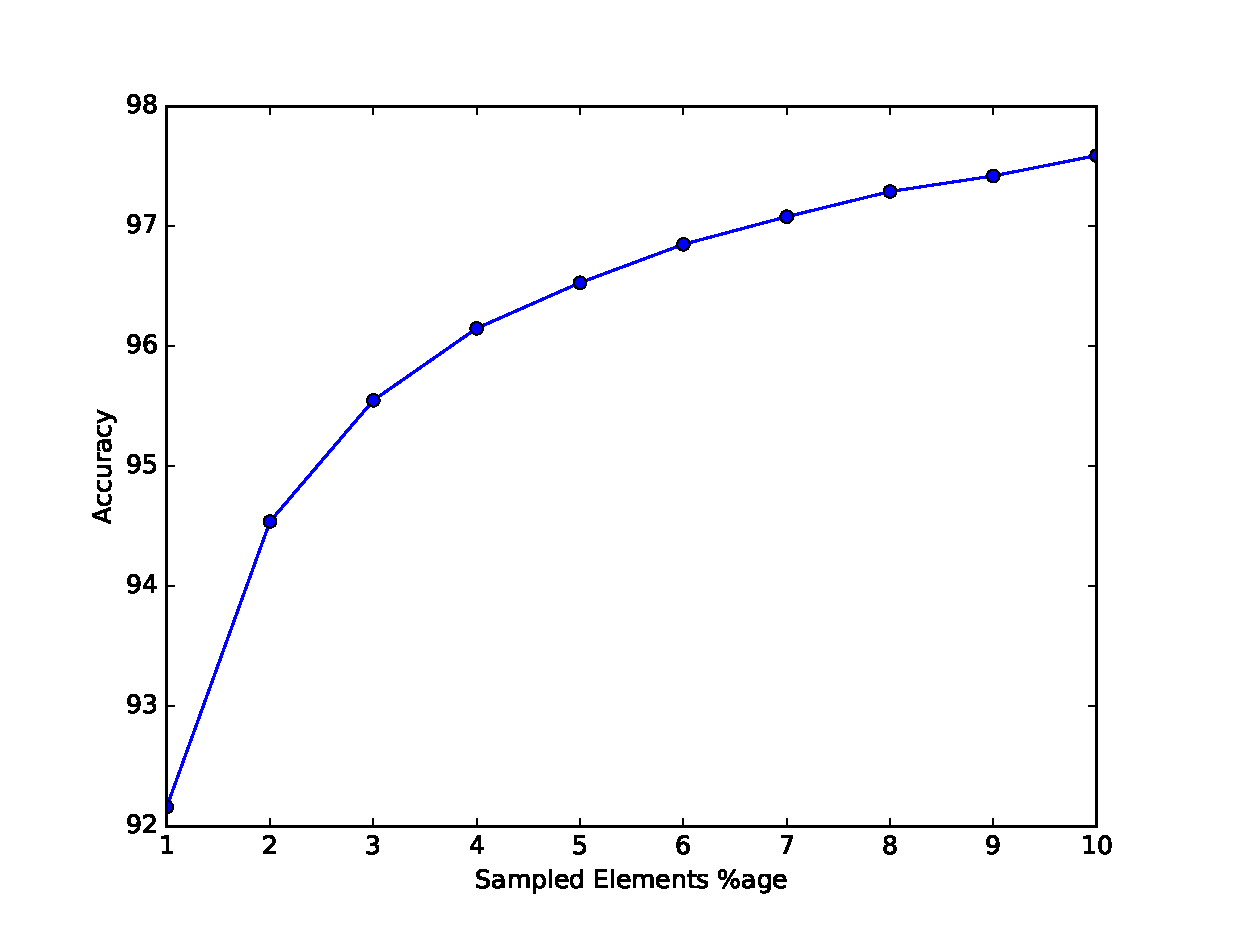
\includegraphics[width=0.95\linewidth]{Results/countnegative1.eps}
  \caption{Accuracy vs Sample Percentage}
  \label{countnegative1}
\end{figure}

\begin{figure}
  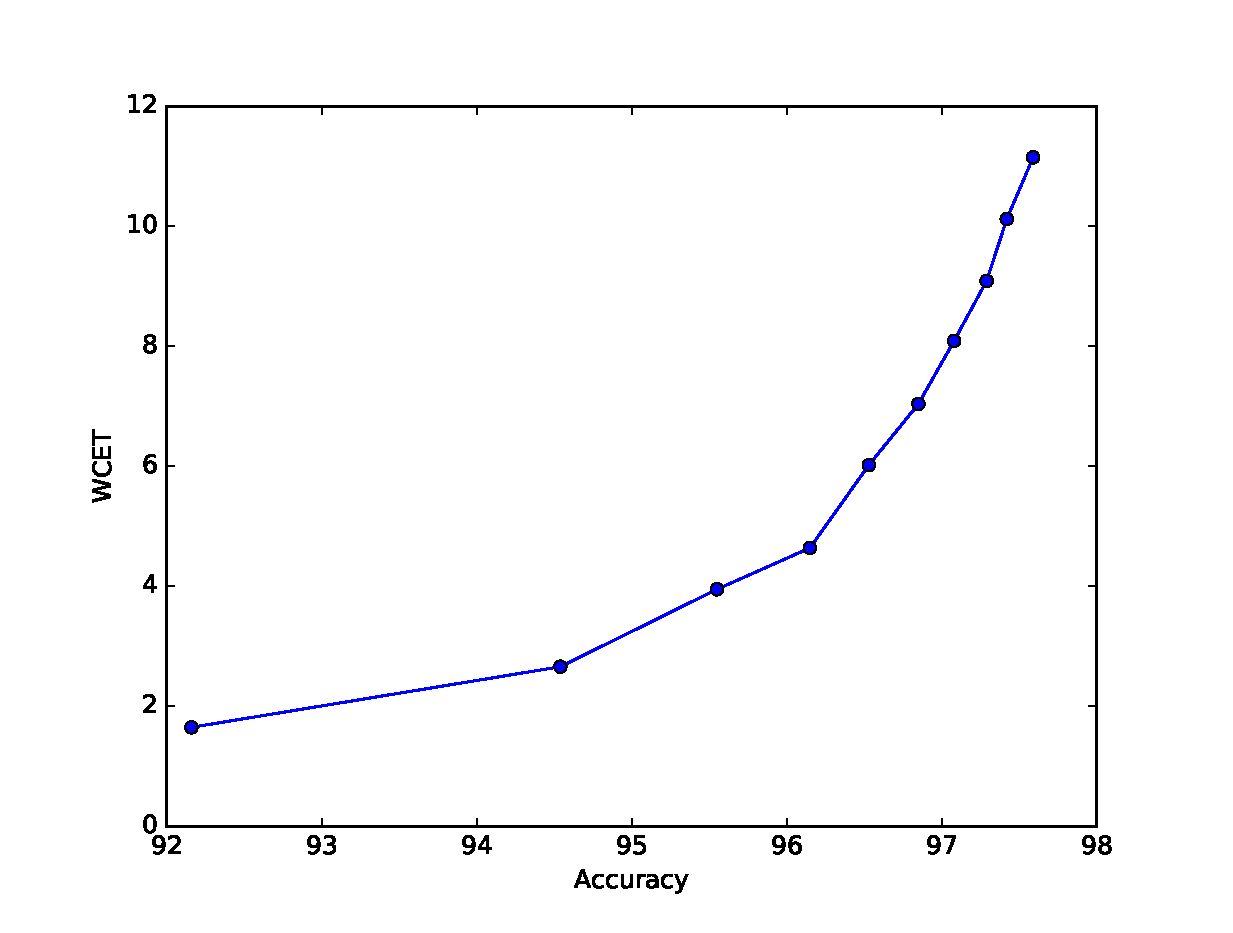
\includegraphics[width=0.95\linewidth]{Results/countnegative3.eps}
  \caption{WCET vs Accuracy}
  \label{countnegative3}
\end{figure}

\begin{enumerate}
\item The accuracy increases rapidly with the increase in sample size. This is clear from figure \ref{countnegative1}. Moreover Table \ref{countnegativeT} clearly shows that the standard deviation decreases with the sample size giving us more confidence in the estimation.
\item The relation between WCET and number of samples used is almost linear. This is expected because of the nature of the code.
\item Figure \ref{countnegative3} shows the almost exponential relation between accuracy and WCET. The graph shows us that by spending almost 11\% of the total time we have already achieved 97\% accuracy. The question a system designer must ask is: Is it worth spending almost 9 times more effort for the remaining 3\% accuracy gain? Considering the nature of the application, if the answer is no then this is a great opportunity to save energy and time.
\end{enumerate}


%% \begin{figure}
%%   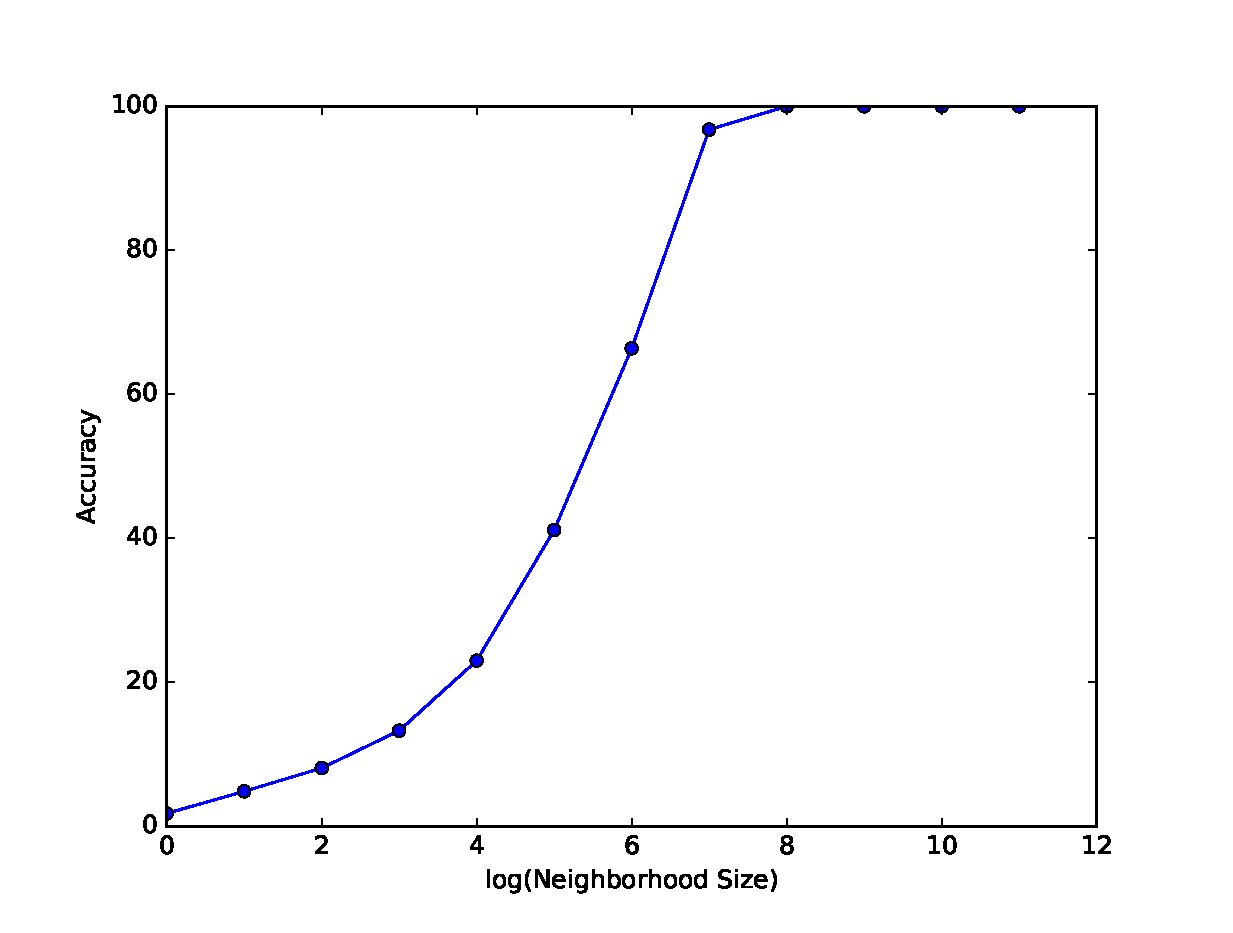
\includegraphics[width=0.95\linewidth]{Results/binarysearch1.eps}
%%   \caption{WCET vs Skipped Iterations)}
%%   \label{binarysearch2}
%% \end{figure}

